\documentclass[a4paper,11pt,DIV=calc,tablecaptionabove,headinclude,twoside]{article}
\usepackage[utf8]{inputenc}
\usepackage{ngerman}
\usepackage{amsmath}
\usepackage{amssymb}
\usepackage{array}
\usepackage{booktabs}
\usepackage{fancyhdr}                   %% Seite, Kopf- und Fußzeile anpassen (siehe \usepackage{geometry})
\usepackage{flafter}                    %% verhindert dass Abbildungen vor Überschrift kommen
\usepackage{float}
\usepackage[pdfpagelabels=true]{hyperref}
\usepackage{geometry}                   %% Seitenmaße verändern (siehe \usepackage{fancyhdr}) !!! Das Paket IMMER nach hyperref einbinden!!!
\usepackage{graphicx}                   %% Einbinden von Bildern mit \includegraphics[]{×}
\usepackage{tabularx}
\usepackage{eurosym}
\geometry{a4paper, top=27mm, left=30mm, right=20mm, bottom=30mm, headsep=10mm, footskip=10mm}
\usepackage[decimalsymbol=comma, binary-units=true, loctolang={DE:ngerman}]{siunitx}
% --------------------------- BibTeX ---------------------------------------
\usepackage[square]{natbib}                 
\bibliographystyle{natdin}           %% Referenzierung: Autor und Jahreszahl
%\bibliographystyle{lex2018}

% Title Page
\title{Experimentplanung LEX 2018}%:\\Messseeelefantenantennenbenennungsverfahren}
\author{Autoren}

\begin{document}
\maketitle



\section{Einleitung}
\subsection{Motivation}
Warum ist das Thema interessant bzw. relevant? Warum lohnt es sich, sich mit dem Thema zu beschäftigen? (0.5--1 Seiten)\\\\
Die Grenzschicht ist der Bereich der Atmosphäre, der direkt vom Boden beeinflusst ist. Dazu zählen bespielsweise der Einfluss von Reibung am Erdboden, Strahlungsprozesse und der generelle Energieaustausch zwischen Boden und Atmosphäre. Die meisten für uns bedeutsamen Wetterparameter, wie bodennahe Temperatur und Wind, die relativen Feuchte oder die Stabilität und Gewitterwahrscheinlichkeit hängen vom Zustand der Grenzschicht ab. Auch wichtige Wetterphänomene, wie die Nebelbildung oder die Land-Seewind Zirkulation finden hier statt.\\
Ein gutes Verständnis und eine präzise Modellierung der Grenzschicht ist jedoch nicht nur für eine gute Wettervorhersage unablässlich, sondern auch beim Bau großer Gebäude, dem Flugverkehr oder für die Optimierung von Windkraftanlagen von Bedeutung.\\
Im Rahmen der LEX bietet sich uns eine einzigartige Möglichkeit, den Aufbau der Grenzschicht in küstennahen Regionen besser zu verstehen, da wir kontinuierliche, zeitlich und vertikal hochaufgelöste in-situ Profilmessungen durchführen können. Von einigen Parametern, wie der Temperatur oder der Feuchte gibt es nur vertikal schlecht aufgelöste Profilmessungen. Durch unsere gute Auflösung selbst in höheren Bereichen der Grenzschicht erhoffen wir uns die Möglichkeit, die zeitliche Entwicklung der Grenzschicht im Messzeitraum besser zu verstehen und möglicherweise sogar neue Erkenntnisse aus diesen abzuleiten.
%\begin{itemize}
	
%	\item Grenzschicht ist die untere Schicht der Atmosphäre, die direkt vom Boden beeinflusst
%	wird
%	\item Reibung, Strahlungsprozesse, Energieaustausch zwischen Boden und Atmosphäre
%	Warum ist die Grenzschicht wichtig? Warum wollen wir sie modellieren?
%	\item  Lebensraum des Menschen
%	\item viele für uns wichtige Wetterparameter hängen vom Zustand der Grenzschicht ab
%	(Temperatur, Feuchte, Nebel, Wind, Land-Seewind Zirkulation, Stabilität)
%	- ausgeprägte tageszeitliche Schwankungen dieser Parameter
%	- wichtig für gute Wettervorhersage
%	- Windkraftanlagen
%	
%	Schwierigkeiten bei der Modellierung/
%	Was fehlt uns zum Verständnis der Grenzschicht?
%	- Turbulenz
%	- zeitliche Entwicklung der Grenzschicht
%	- Mischprofile Land/See (wichtig für Modelle, Gitterpunkte mit Land und See)
%\end{itemize}
%
%
%Kontinuierliche zeitlich und vertikal hochaufgelöste in-situ Messungen der
%atmosphärischen Grenzschicht bis 1000m Höhe existieren bislang nur sporadisch.

\subsection{Wissenschaftliche Ziele/Fragen}
Jedes Ziel mit Bullet-Punkten kurz und prägnant definieren; ein bis zwei -- auch stichwortartige -- Sätze genügen; nach Möglichkeit Hypothesen/Fragen formulieren, die im Experiment überprüft/beantwortet werden sollen. (wenige, 1 bis 5 Ziele)

\begin{itemize}
%\item Entwicklung der 'Hardware', um Profilmessungen der Grenzschicht mithilfe eines Fesselballons oder eines Drachens von Temperatur und Feuchte (mit möglichst hoher vertikaler Auflösung) durchführen zu können.
%\item Welche Sensoren eignen sich? Interne Variabilität, absolute Genauigkeit
%\item Grenzen der Messmethoden prüfen: Wie geeignet ist der Fesselballon/Drachen/Drohne für welche Zwecke: ZIEL: Wie kann man die Messungen beider (aller drei) Messmethoden ideal kombinieren, um möglichst viele Informationen zu erhalten. Vertikalauflösung und zeitliche Auflösung der Arduinos, was sind die Möglichkeiten der Messung durch die Drohne, was sind die Grenzen?
%\item Wie sehr beeinflusst der Downwash der Drohne die Messungen?
%\item Drohne: Messungen über dem Meer: \textbf{Unterschied Grenzschicht Land Meer}, Entwicklung der Grenzschicht über Land, wie weit reicht der Einfluss des Meeres/Landes
%\item Zeitskalen: Wie schnell entwickeln sich die neue Grenzschicht? Z.B., wenn sich die Anströmrichtung von Land auf Meer wechselt
\item Entwicklung und Test einer eigenen Messhardware zur Profilmessung von
    Temperatur, Feuchte und Druck
\item Wie entwickelt sich die morgentliche Grenzschicht? Auf welchen Zeitskalen spielt sich diese Entwicklung ab?
\item Wie beeinflusst die Anströmrichtung die Profile über der Insel? Ist ein
    Landseewind erkennbar?
\end{itemize}

\section{Stand der Forschung}
Was ist zum Thema bekannt? Welche Vorarbeiten (Paper, alte LEX-Berichte usw.) gibt es, an die angeknüpft werden kann?\\
- Übergang Tag-/Nachtgrenzschicht (Theresa)\\ % nur allgemeine Beschreibung, was erwarten wir?
- Übergang Land-/Seegrenzschicht (Henning)\\ % nur allgemeine Beschreibung
- In ... wurden bereits Beobachtungen in einer ähnlichen Umgebung (küstennah, auf einer Insel) mit ähnlichen Messmethoden (Ballon, Drohne) erfolgreich durchgeführt.  

- Gibt es Grenzschichtmessungen mit einem ähnlich hohen Ballon? (Simi)

Aufgrund ihrer Flexibilität und dem relativ niedrigen Anschaffungspreis werden
in den letzten Jahren immer häufiger Drohnen für Messungen in der atmosphärischen
Grenzschicht verwendet.
\citet{kunz2018cocap} haben zum Beispiel COCAP entwickelt, ein Gerät zur Messung von
CO2, das spezialisiert ist, um mit Drohnen zu fliegen. Die Temperatur und Feuchtesensoren
von COCAP werden dabei unter den Rotoren der Drohne befestigt, sodass sie durch die 
Zugluft der Rotoren belüftet werden. \citet{jimenez2016morning} führten Messungen der morgentlichen Grenzschicht
auf Mallorca durch und fanden ebenfalls gute Übereinstimmung mit Wetterstationen, 
Ballonmessungen und mesoskaligen Modellen. Hierbei waren die Sensoren über den Rotoren
der Drohne befestigt.\\
Zum Einfluss des Downwash-Effektes einer Drohne auf die Messungen gibt es bisher
wenig Erkenntnisse. \citet{zhou2017small} befand nach Testmessungen den Einfluss für
minimal.\\

- Sensoren:





\section{Messstrategie}
Wie sieht die allgemeine Messstrategie aus? Welche Größen sollen z.~B. mit welcher zeitlichen Auflösung gemessen werden, um die wissenschaftliche Fragestellung beantworten zu können?

Im Rahmen des Experimentes soll untersucht werden, wie sich die Größen Temperatur, Feuchte und Druck in der Grenzschicht im Verlauf eines Tages entwickeln, wobei besonderer Fokus auf den Übergang zwischen nächtlicher und konvektiver Grenzschicht gelegt werden soll. Zusätzlich sollen Erkenntnisse darüber gewonnen werden, ob und wie die küstennahe Grenzschicht durch die unmittelbare Nähe zum Meer beeinflusst wird und wie sich unterschiedliche Anströmrichtungen auswirken. 

Die Kombination von zwei Messstrategien soll dies ermöglichen: Zur Beobachtung der zeitlichen Entwicklung werden mithilfe eines Helikites ab täglich ab Sonnenaufgang bis zum Nachmittag die Größen Temperatur, Feuchte und Druck in 10 Messhöhen zwischen dem Boden und 1000\,m mit einer zeitlichen Auflösung von 1\,s gemessen.
Zusätzlich ist geplant ein Lidar in der Nähe des Helikites zu installieren, mit dem Vertikalprofile von Windgeschwindigkeit und -richtung in hoher zeitlicher Auflösung gemessen wird. % Welche Auflösung usw.?
Um den Einfluss des Meeres auf die küstennahe Grenzschicht zu verstehen, soll zusätzlich eine Drohne verwendet werden, mit der zwei mal täglich instantane Horizontalprofile der Messgrößen über Land und Meer in mindestens zwei Messhöhen zwischen dem Boden und 100\,m Höhe gewonnen werden. 

\subsection{Experimenteller Aufbau}
\label{Aufbau}
%Welche Instrumente sollen wie (Messhöhe, Standortwahl, horizontale Abstände, ... ) aufgebaut werden? (nach Möglichkeit Skizzen und Pläne hinzufügen)
%- 1km Messhöhe
%- im Idealfall (Ballonschnur vertikal): 2, 20, 50, 100, 280, 460, 640, 820,1000 %TODO: nochmal nachdenken, Skizze machen
%- Standort: Welcher Ort ist genehmigt? -> Hubschrauberlandeplatz (ca. 70m vond er Küste entfernt, keine Bäume)
%
%- Welche Instrumente?: Temperatur, Feuchte, Druck an Arduino
%
%- Drohne: Sensor unterhalb der Drohne (ca. 20cm) befestigt. Es sollen 2D profile als Ergänzung zum Ballon geflogen werden %TODO: Wie genau soll mit der Drohne geflogen werden?
%
%- Arduinos senden Daten live: Aufbau: Slaves/Master

Um die beschriebene Messstrategie umsetzen zu können, werden Messinstrumente an einem Helikite und an einer Drohne befestigt. 
Der Helikite hat ein Volumen von 14\,$\text{m}^{3}$, eine Nutzlast von 4\,kg und kann auf eine Höhe von bis zu 1000\,m steigen. Er wird auf dem Hubschrauberlandeplatz des Bundeswehrgeländes in Marienleuchte in ca. 80\,m Entfernung zur Küste (Abbildung) fest am Boden verankert. Nur für diesen Standort wurde eine entsprechende Aufstiegsgenehmigung beantragt. An der Leine des Helikites werden insgesamt 10 Messinstrumente in unterschiedlichen Abständen befestigt (Abbildung). Geplante Messhöhen sind 2\,m, 20\,m, 50\,m, 100\,m, 180\,m, 300\,m, 450\,m, 620\,m, 820\,m und 1000\,m, sodass die Abstände im unteren Bereich der Grenzschicht enger liegen als im oberen. Diese Abstände werden womöglich nicht exakt einzuhalten sein, da an der Leine des Helikites in bestimmten Abständen zusätzliche Markierungen befestigt werden müssen, die der Sichtbarkeit dienen. Die tatsächlichen Messhöhen lassen sich dann anhand des gemessenen Drucks bestimmen. \\

Sollte ein Aufsteigen des Helikites aufgrund der Wetterbedingungen nicht möglich sein (siehe Abschnitte \ref{Bedingungen} und \ref{Risiken}), wird anstelle dessen bei niedrigen Windgeschwindigkeiten ein Fesselballon installiert, bei hohen Windgeschwindigkeiten ein Drachen. Die Messinstrumente werden in diesem Fall in äquidistanten Abständen bis zur maximal möglichen Messhöhe angebracht. \\
  
Alle Instrumente bestehen aus einem Arduino Board, einem BME280 Sensor zur Messung von Druck, Temperatur und relativer Feuchte und einem Long Range Wide Area (LoRa) Modul, das zur sofortigen Übermittlung der Daten zum sogenannten 'Master' am Boden dient (Foto). Eine Übersicht über die technischen Daten des BME280 befindet sich in Abbildung \ref{BME_280}. Die Stromversorgung der Instrumente erfolgt mit Powerbanks mit einer Kapazität von 2000 mAh. Dies reicht auch bei maximalem Stromverbrauch der Messinstrumente für einen Tag. Das oberste Instrument, das unmittelbar unterhalb des Ballons befestigt wird, verfügt zusätzlich über ein GPS Modul, sodass sich die Neigung der Leine aufgrund des Winds feststellen lässt. Die Instrumente werden in einem Rohr aus Acrylglas verpackt. Die einzelnen Bauteile werden dort so befestigt, dass sich nicht durch Stöße beschädigt werden können. Der Messsensor befindet sich außerhalb des Rohrs. So wird erreicht, dass der Sensor gut belüftet ist und verhindert, dass die Messungen durch ein strahlungsbedingtes Aufheizen oder Abwärme der anderen Komponenten innerhalb des Rohrs beeinflusst werden.  
Jedes der Messgeräte inklusive Verpackung und Befestigungsvorrichtung wiegt ca. 200\,g, sodass das Gesamtgewicht deutlich unter der Nutzlast des Helikites liegt.\\
   
Ein weiteres Messgerät gleicher Bauart (mit GPS Modul) wird direkt an der Unterseite einer Drohne des Typs DJI Phantom 2 befestigt. Diese kann eine Nutzlast von maximal 500\,g transportieren und hat eine Flugdauer von ca. 10 Minuten. Sie kann eine Maximalgeschwindigkeit von 15\,m/s erreichen, was somit gleichzeitig der maximalen Einsatzwindgeschwindigkeit entspricht. Das geplante Flugmuster der Drohne wird in Abschnitt \ref{sec:Durchfuehrung} beschrieben. \\

Ein Lidar der Firma METEK wird ebenfalls auf dem Gelände der Bundeswehr installiert. Genaue Angaben zu vertikaler und zeitlicher Auflösung können zum jetzigen Zeitpunkt noch nicht gemacht werden, da wir noch keine Informationen zum Lidar erhalten haben.  


\begin{figure}
\centering
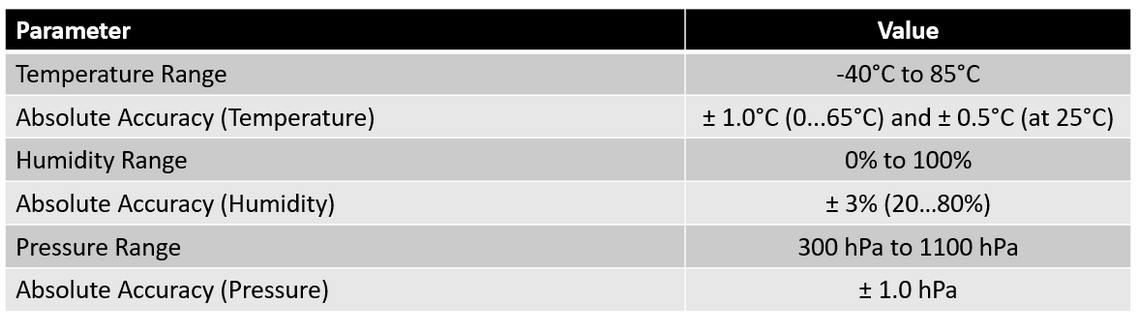
\includegraphics[width=\textwidth]{BME_280_technische_Daten.png}
\caption{Technische Daten des BME280 Sensors}
\label{BME_280}
\end{figure}

\subsection{Bedingungen/Erfordernisse}
\label{Bedingungen}
%Welche externen Bedingungen sind notwendig (Wetter)? Welche internen Erfordernisse sind notwendig (Betriebsmittel, Personal, externe Daten zur Durchführung usw.)? Sind Messdaten der anderen Gruppen erforderlich (Messstrategie absprechen)?

Folgende externe und interne Erfordernisse sind notwendig, um die geplanten Messungen erfolgreich durchführen zu können.

\subsubsection{Externe Bedingungen}

Die wichtigste externe Voraussetzung ist die Wetterlage, da die Messungen nicht bei Niederschlag durchgeführt werden können. Wie in Abschnitt \ref{Aufbau} beschrieben, ist der Sensor nicht wie der übrige Teil der Messgeräte durch eine Verpackung geschützt. Er sollte jedoch auf keinen Fall mit Wasser in Berührung kommen, um eine Beschädigung der Elektronik zu verhindern. Gleiches gilt auch für die Drohne. Auch bei hohem Niederschlagsrisiko kann das Experiment nicht durchgeführt werden. \\

Für die Messungen mit der Drohne spielt die Windgeschwindigkeit eine wichtige Rolle. Das verwendete Modell kann laut Hersteller bis zu einer maximalen Windgeschwindigkeit von 15\,m/s geflogen werden. Wir rechnen jedoch damit, dass es nur bis zu deutlich geringeren Windgeschwindigkeiten (ca. 5\,m/s) möglich ist, die Drohne mit ausreichender Sicherheit und Genauigkeit zu steuern. \\

Auch für den Helikite müssen bestimmte Windbedingungen vorherrschen. Genaue Angaben zu maximalen oder minimalen Windgeschwindigkeiten können noch nicht gemacht werden, wir gehen jedoch davon aus, dass der Helikite auch für hohe Windgeschwindigkeiten ausgelegt ist. \\

\subsubsection{Interne Bedingungen}

Um den Helikite wie geplant einsetzen zu dürfen, ist eine behördliche Genehmigung nötig. Eine solche Genehmigung wurde für einen Aufstiegszeitaum zwischen Sonnenaufgang und Sonnenuntergang und für eine maximal Aufstiegshöhe von 1000\,m bereits beantragt. Bisher haben wir jedoch noch keine Rückmeldung erhalten.\\

Sowohl die Drohne als auch die Messinstrumente werden über Akkus mit Strom versorgt, die zwischen den Messphasen geladen werden müssen. In der Nähe des Messstandortes müssen deshalb ausreichend USB-Ladekabel und Steckdosen vorhanden sein.\\

Es muss damit gerechnet werden, dass es bei den Messinstrumenten zu Ausfällen kommt. Es müssen deshalb ausreichend Ersatzteile und Werkzeuge bereit liegen, um kaputte Bauteile möglichst schnell ersetzen zu können. Die Software der Messgeräte kann in Form sogenannter Sketches nur über einen PC auf den Arduino aufgespielt werden, sodass auch PCs mit der benötigten Software vorhanden sein müssen.\\

Für den Helikite bzw. den Ballon wird ausreichend Helium benötigt. Zudem muss für die Winde des Helikites am Messstandort (Helikopterlandeplatz) eine Stromversorgung vorhanden sein. \\
 

%\begin{itemize}
%\item externe Bedingungen:
%	\item kein Niederschlag, auch keine Niederschlagwahrscheinlichkeit!
%	\item max. Wind für Ballon %TODO Felix fragen
%	\item max. Wind für Drohne: theoretisch 15m/s, wir schaffen es nur bis geringe Windgeschwindigkeit (max. 5m/s)
%	\item für Land-Seewind: möglichst wenig Wind\\
%	
%\item interne Erfordernisse:
%	\item Kine anderen Messungen erforderlich
%	\item Helikite
%	\item Drohne
%	\item Flugerlaubnis
%\end{itemize}

\subsection{Durchführung}
%Beschreibung des regulären Messablaufs. Sind Intensivmessphasen geplant? Auf welche besonderen Ereignisse soll wie reagiert werden? 
%Wann werden zusätzliche Messungen (z.\,B. Radiosondenaufstiege) durchgeführt?
%Wie sollen die Messdaten aufgezeichnet werden? \\

%\textbf{Reguläre Durchführung:}\\
%\begin{itemize}
%\item Ab Sonnenaufgang (06:15, 28.08; 06:35, 08.09) muss gemessen werden. Ballon schon vorher aufgebaut werden: Tag 1: 2h für Aufbau planen, alle. Anschließend anpassen (kürzere Vorbereitungszeit, evtl. weniger Leute, je nachdem, wie schnell wir sind.
%\item Messzeitraum: Sonnenaufgang bis 15Uhr. Dann soll der Ballon unten sein.
%\item durchgehende Messungen von T, Rh, p. In Auflösung: sekündlich.
%\item Daten werden in Echtzeit an Master gesendet, können während des Messzeitraums ausgewertet werden.
%\end{itemize}
%
%\textbf{Zusätzliche Drohnen-Messungen :}\\
%Es sind Intensivmessphasen mit der Drohne geplant.
%\begin{itemize}
%\item Zwei Drohnenmessungen täglich, wenn die Grenzschicht schon aufgebaut ist.
%\item Winkel zum Wind: parallel zum Wind)
%\item Welche Form soll die Drohne fliegen?: Einmal 250m raus aufs Meer, einmal zurück in anderer Höhe und auf dieser Höhe weiter übers Land (insg. 500m), in neuer Höhe zurück (250m). Falls Akku leer, hier Messstop. Sonst nochmal über Meer in dieser Höhe (insg. weitere 500m). (Also Stufenprofil)
%\item Evtl. Zusatzmessungen bei besonderen Ereignissen.
%\end{itemize}

Der reguläre Messtag startet ca. 1 bis 2 Stunden vor Sonnenaufgang, der im zwölftägigen Zeitraum der Messkampagne zwischen 6:15 Uhr (28.08.2018) und 6:35 Uhr (08.09.2018) stattfindet. Der Helikite muss bis zum Sonnenaufgang vollständig aufgebaut sein. Am ersten Tag planen wir für den Aufbau des Helikites 2 Stunden ein und das gesamte Team ist anwesend. Je nachdem, wie lange der Aufbau dauert können Zeit und Personenanzahl an den Folgetagen angepasst werden. Nach einer Überprüfung der Wetterlage entscheidet das Team, ob ein Aufstieg möglich ist. Während des Aufbaus müssen die Messinstrumente an ihre Powerbanks angeschlossen werden und auf Funktionalität geprüft werden. Anschließend werden sie in den in Abschnitt \ref{Aufbau} genannten Abständen an der Leine des Helikites befestigt, während wir diesen aufsteigen lassen. \\

Sobald die Messinstrumente mit Strom versorgt sind werden ihre Messdaten in sekündlichen Abständen an den Master am Boden gesendet. Neben den Messwerten wird auch eine individuelle Kennung verschickt, die es ermöglicht, die empfangenen Daten dem jeweiligen Messinstrument zuzuordnen. Der Master ist an einen PC angeschlossen, mit dem die empfangenen Daten direkt ausgelesen und abgespeichert werden können. Außerdem werden die Profile von Temperatur, Feuchte und Druck live geplottet. So kann auf interessante oder unerwartete Entwicklungen reagiert werden und eventuell zusätzliche Messungen mit der Drohne gewonnen werden.\\

Planmäßig sollen Messungen bis ca. 15 Uhr stattfinden, danach wird der Helikite abgebaut. Das Wetter wird jedoch während des gesamten Messzeitraums beobachtet und es wird sofort mit dem Abbau begonnen, sobald sich Niederschlag oder eingeschränkte Sichtverhältnisse ankündigen. Während die Leine eingeholt wird, werden die einzelnen Instrumente abgenommen, gesammelt und ihre Powerbanks anschließend aufgeladen. \\

Zweimal täglich finden Messungen von Horizontalprofilen mit der Drohne statt. Die erste Messung findet unmittelbar nach Sonnenaufgang statt, die zweite am frühen Nachmittag. Dadurch erhoffen wir uns, die Grenzschicht in möglichst verschiedenen Zuständen zu beobachten.  
Der Bereich, der mit der Drohne abgeflogen werden kann ist dadurch limitiert, dass laut Vorschrift maximal bis zu einer Höhe von 100\,m und nur auf Sicht geflogen werden darf. Zusätzlich hat die Drohne nur eine begrenzte Akkulaufzeit von ca. 10 Minuten. Abbildung ... zeigt das geplante Flugmuster. Da die Messungen Erkenntnisse darüber liefern sollen, ob und wie die Nähe zum Meer die küstennahe Grenzschicht beeinflusst, sollen die Horizontalprofile sowohl über Land als auch über Wasser aufgenommen werden.
Die Drohne wird in ausreichendem Abstand zum Helikite gestartet und auf eine Höhe von ca. 20\,m gebracht. Anschließend soll sie senkrecht zur Küstenlinie über die Küste hinaus und über das Meer fliegen. Die Flugrichtung wird beibehalten, bis die Drohne sich ca. 250\,m vor der Küste befindet, wenn das Sichtfeld diese Entfernung erlaubt. Bevor die Drohne zurück fliegt erfolgt ein Aufstieg auf ca. 50\,m. Sobald die Drohne ca. 250\,m landeinwärts zurück gelegt hat, erfolgt ein erneuter Aufstieg und die Drohne fliegt zurück zum Ausgangspunkt. Ist der Akkuladung zu diesem Zeitpunkt noch ausreichend hoch, kann ein weiteres Profil über dem Meer geflogen werden (s. Abbildung), ansonsten wird die Drohne gelandet.   
- Wie wird kalibriert (1. Tag)
- Wann, wie und ob werden Drache/Ballon eingesetzt
- Gibt es weitere einmalige Messungen?

\subsection{Auswertung}
Wie sollen die Daten ausgewertet werden? Sind zusätzliche Daten (Satellitendaten, Modelldaten usw.) notwendig? Welche Grafiken oder Auswertungen sollen im Idealfall am Ende die wissenschaftlichen Fragen beantworten?\\

Zum Test der Messhardware (Helikite und Drohne) werden eines oder mehrere gemessene Profile 
mit gleichzeitigen Messungen einer Radiosonde verglichen. Zur Auswertung werden beide Profile
in einem Plot dargestellt und vergleichend analysiert.\\
Zur Untersuchung der Entwicklung der Grenzschicht werden entweder gemessene Profile zu verschiedenen 
Zeiten in einen Plot Höhe gegen Temperatur/Feuchte/(Wind) aufgetragen oder eine komplette Messreihe in einen 
2-D Konturplot Zeit-Höhe-Temperatur/Feuchte/Wind aufgetragen. So lassen sich Veränderungen der Grenzschicht sowie
deren Zeitskalen analysieren, eventuelle Land-See-Wind-Regimes identifizieren und Veränderungen aufgrund eines 
Wechsels der Anströmrichtung erkennen.\\
Unterschiede der Grenschicht über Land und Meer werden durch eintragen der von der Drohne gemessenen Profile 
in einen gemeinsamen Plot identifiziert.\\

\subsection{Risiken}
\label{Risiken}
Woran könnten Teile des Experiments scheitern? Welche Alternativen gibt es in diesen Situationen? (für jedes Risiko einen Absatz)\\

Die Benutzung des Helikites bis in 1000 m Höhe ist, wie oben beschrieben, an eine
Wetterlage mit guter Sicht bis in 1000 m ohne Sturm/stürmischen Wind gebunden. Falls diese Bedingungen nicht erfüllt werden, muss
auf das Helikite verzichtet werden. In diesem Fall wird auf Messungen mit einem Ballon und/oder Drachen 
zurückgegriffen. Diese fliegen nur bis etwa 100-200 m. Dementsprechend würde sich die Analyse der Grenzschicht 
nur auf diese Höhen beziehen. Die Sensoren könnten demensprechend in kürzerem Abstand aufgehangen werden.\\
Die entwickelten Sensoren sind nicht wasserfest und somit bei Niederschlag nicht einsetzbar. Bei 14 Tage Regen am Stück
würde das Experiment scheitern. In diesem Falle wäre eine Alternative, die Grenzschicht mit möglichst vielen Radiosondenaufstiegen
zu untersuchen. \\
Auch die Messung der Windprofile mit dem Lidar hängt von der Wetterlage ab, da nur bis zur Wolkenunterkante gemessen werden kann. \\
Es besteht das Risiko, dass ein oder mehrere Sensoren ausfallen. Ein Ausfall des Masters am Boden wäre am
schlimmsten, da dann keine Kommunikation mehr mit den anderen Sensoren möglich ist. Für den Fall von 
Sensorausfällen sind für beide Arduino-Typen mindestens ein Ersatz eingeplant. Auch für die LoRa Chips und für
die BME280-Sensoren ist Ersatz vorhanden, der bei Ausfall zum Einsatz kommt.\\

\section{Kosten}
Kosten für zusätzliches Material, Geräte, Betriebsmittel ...\\
Die Materialkosten sind in Tabelle \ref{Tab:Kosten} aufgelistet.
\begin{table}[h]
\caption{Auflistung der Materialkosten}
\begin{tabular}{|c|c|c|c|}
\hline
Gegenstand (?) & Preis (\euro) & Anzahl & Gesamtpreis (\euro) \\\hline \hline
RFM95W Lora Module 868MHz  & ?? & 12 & ?? \\\hline
Dragino Lora Shield 868MHz & 22 & 1 & 22 \\\hline
Arduino Nano & ?? & 10 & ?? \\\hline
Arduino Uno & ?? & 2 & ?? \\\hline
Dragino Lora/GPS Shield 868MHz & 35 & 1 & 35 \\\hline
Jumper Kabel male female & 0,2? & 100 & 20? \\\hline
Powerbank & 3,99 & 13 & 51,87 \\\hline
USB Kabel & 0,95 & 13 & 12,35 \\\hline
Bluedot BME280 Sensor & 17 ? & 17 & 289? \\\hline
Lochrasterplatinen Hartpapier 500x100mm H25PR500 & 6,45 & 3 & 19,35 \\\hline
\end{tabular}
\label{Tab:Kosten}
\end{table}

\section*{Literatur}
\bibliography{Whitepaper}
\end{document}